%template1.tex
%The following LaTeX source file represents the simplest kind of slide presentation; no overlays, no included graphics. Substitute your favorite style for ``pascal''. To create the PDF file template1.pdf, (1) be sure to use the prosper class, then (2) execute the command latex template1.tex, and (3) the command dvipdf template1.dvi.

%%%%%%%%%%%%%%%%%%%%%%%%%%%%%%% template1.tex %%%%%%%%%%%%%%%%%%%%%%%%%%%%%%%%%%%
\documentclass[a4paper,blends,pdf,colorBG,slideColor]{prosper}
% definitions for slides for CSC544
% Lutz Hamel, (c) 2007

\hypersetup{pdfpagemode=FullScreen}

\usepackage{times}
\usepackage{latexsym}
\usepackage{alltt}
\usepackage{booktabs}
\usepackage{amsmath}
\usepackage{amsopn}
\usepackage{amsfonts}
\usepackage{amssymb}
%\usepackage[usenames]{color}

\def\sign{\qopname\relax{no}{sign}}
\def\argmax{\qopname\relax{no}{argmax}}
\def\argmin{\qopname\relax{no}{argmin}}

\newcommand{\grad}{\ensuremath{\nabla}} 
\newcommand{\loss}{\ensuremath{{\cal L}}}
\newcommand{\err}{\mbox{err}}
\newcommand{\mse}{\mbox{mse}}
\newcommand{\acc}{\mbox{acc}}
\newcommand{\Integer}{\ensuremath{\mathbb{N}}}
\newcommand{\size}[1]{{|{#1}|}}
\newcommand{\Rnspace}[1]{\ensuremath{\mathbb{R}^{#1}}}
\newcommand{\Real}{\ensuremath{\mathbb{R}}}
\newcommand{\mytt}[1]{{\small\tt{#1}}}
\newcommand{\textemph}[1]{{\em #1}}
\newcommand{\suchthat}{\mid}
\newcommand{\orbar}{\;|\;}
\newcommand{\bs}[1]{\begin{slide}{#1}\ptsize{8}}
\newcommand{\es}{\end{slide}}
\newcommand{\co}{\,\colon\;}
\newcommand{\pair}[2]{\ensuremath{( {#1}, {#2} )}}
\newcommand{\model}[1]{\hat{#1}}
\newcommand{\ul}[1]{{\bf\em #1}}
\newcommand{\ol}{\overline}
\newcommand{\definition}[1]{{\bf Definition: }{\em #1}}
\newcommand{\example}[1]{{\bf Example: }{#1}}
\newcommand{\abs}[1]{|{#1}|}
\newcommand{\mytab}{\makebox[.1in]{}}

\newcommand{\fdef}[1]{
\begin{center}
\fbox{
\begin{minipage}{3.5in}
{\bf Definition:}
{#1}
\end{minipage}
}
\end{center}
}

\newcommand{\fframe}[1]{
\begin{center}
\fbox{
\begin{minipage}{3.5in}
{#1}
\end{minipage}
}
\end{center}
}

\newcommand{\nframe}[1]{
\begin{center}
\begin{minipage}{3.5in}
{#1}
\end{minipage}
\end{center}
}

\newenvironment{Rcode}
	{
		\scriptsize
		\begin{quote}
		\begin{alltt}
	}
	{
		\end{alltt}
		\end{quote}
	}




\begin{document}
\bs{Welcome - CSC 581}
\begin{center}
	{\LARGE\em Introduction to Machine Learning with Support Vector Machines}\\

	Dr. Lutz Hamel\\
	hamel@cs.uri.edu\\
	Tyler Hall, Rm 251\\
	\vspace{.3in}

    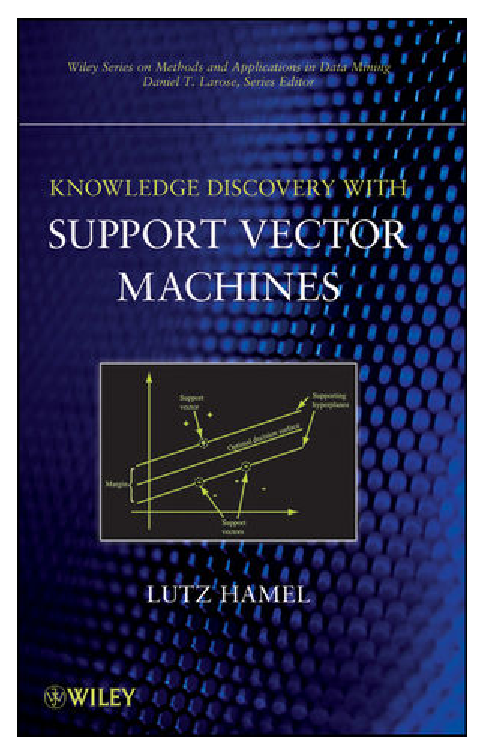
\includegraphics[height=35mm]{images/bookcover.eps}
\end{center}

\es

\bs{Reference Material:}

We will be using my book {\em Knowledge Discovery with Support Vector Machines}, Hamel, Wiley, 2009.

Other books of interest:
\begin{itemize}
\item
{\em Introductory Statistics with R}, Peter Dalgaard, Springer, 2008.
\item
{\em Pattern Recognition and Scene Analysis}
Richard Duda, Peter Hart, Wiley, 1973.
\item
{\em The Elements of Statistical Learning}, 2ed, Jerome Friedman, Trevor Hastie\
, and Robert Tibshirani, Springer, 2016.
\item
{\em Learning with Kernels}, Berhard Schoelkopf and Alexander Smola, MIT Press,\
 2002.
\item
{\em  Neural Networks for Pattern Recognition},  Christopher M. Bishop, Oxford \
University Press, 1995.
\end{itemize}
\es

\bs{Knowledge Discovery}
\begin{center}
    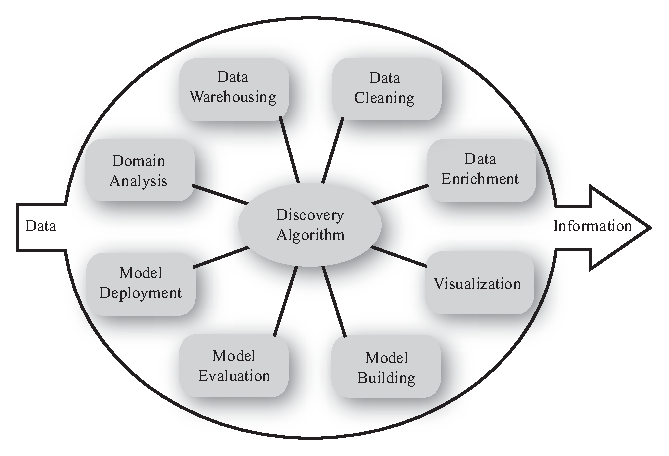
\includegraphics[height=40mm]{figures/fig01-01.eps}
\end{center}

\begin{itemize}
\item Semi-automated process of extracting useful information from collections of data.
\item Computer-based tools for the discovery process but that
guidance by an analyst is indispensable.
\item Highly interdisciplinary.
\item Data Mining - Knowledge Discovery in Databases (KDD)
\end{itemize}
\es

\bs{Machine Learning}

From our perspective, machine learning is at the core of knowledge discovery.

A qualitative definition of machine learning:

\begin{quote}
Programs that get better with experience given a task and some performance measure.
\end{quote}
\es


\bs{Machine Learning}

A more quantitative definition of machine learning:
\begin{quote}

Given
\begin{itemize}
\item A data universe $X$.
\item A sample set $S$ where $S \subset X$.
\item Some target function (labeling process) $f\co X \rightarrow \{\text{\it true}, \text{\it false}\}$.
\item A labeled training set $D$, where
$
D = \{ (x ,y) \suchthat x \in S \text{ and } y = f(x)\}.
$
\end{itemize}
Compute a function $\model{f}\co X \rightarrow \{ \text{\it true}, \text{\it false}\}$ using $D$ such that,
\begin{equation*}
\label{eq:process-model}
\model{f}(x) \cong f(x),
\end{equation*}
for all $x \in X$.
\end{quote}

This definition of machine learning is referred to as {\em supervised learning}
due to the fact that the algorithm needs a labeled dataset $D$.

{\bf Observation:} We can view the function $\model{f}$ as a {\em model} or {\em approximation}
of the original function $f$.  The model is computed only based on the 
observations in the training dataset $D$.
\es

\bs{Inductive Reasoning}
The fundamental assumption in machine learning is that the training  set $D$
is an accurate representation of the whole data universe $X$.

\begin{quote}
{\bf The Inductive Learning Hypothesis:} \it Any function found to approximate the 
target function well over a sufficiently large training set $D$ will 
also approximate the target function well over the data universe $X$.
\end{quote}

\es

\bs{But...}
Inductive reasoning has its pitfalls, as can be demonstrated with the classic black
swan problem.
\begin{center}
    \includegraphics[height=40mm]{figures/fig01-02.eps}
\end{center}
That is, if your training set $D$ is not representative of the data universe $X$ then
your model, in this case "all swans are white", will most likely not be correct.
\es

\bs{The Universe $X$}
A convenient way to describe objects in a data universe $X$ is by the use of a {\em feature table}.

\begin{center}
{\small
   \begin{tabular}{ l cccc}
      \toprule
         & Legs & Wings & Fur & Feathers\\
      \midrule
      cat      & 4 & no & yes & no \\
      crow      & 2 & yes & no & yes \\
      frog      & 4 & no & no & no \\
      bat      & 4 & yes & yes & no \\
     barstool      & 3 & no & no & no \\
      \bottomrule
   \end{tabular}
   }
\end{center}

\begin{itemize}
\item Each labeled column in the table is called an {\em attribute}.
\item Each labeled row is an object of the universe.
\item This is only a subset of all possible objects that can be described with the attributes (sample set).
\end{itemize}
\es

\bs{The Universe $X$}
Let $\text{\it mammal}\co X \rightarrow \{\text{\it true}, \text{\it false}\}$ be a target function, then
we can convert our feature table into a training set by (a) dropping the names of the objects and (b) adding a column with the labels generated by $\text{\it mammal}$:

\begin{center}
{\small
   \begin{tabular}{ccccc}
      \toprule
        Legs & Wings & Fur & Feathers&Mammal\\
      \midrule
     4 & no & yes & no& {\it true} \\
      2 & yes & no & yes & {\it false}\\
      4 & no & no & no & {\it false}\\
     4 & yes & yes & no & {\it true}\\
     3 & no & no & no &{\it false}\\
      \bottomrule
   \end{tabular}
}
\end{center}
A reasonable model $\model{f}$ for $\text{\it mammal}$ based on this training set is,
\begin{equation*}
\model{f}(\text{\it legs}, \text{\it wings}, \text{\it fur},\text{\it feathers}) \equiv \text{ \bf if } \text{\it fur} = \text{ yes } \text{ \bf then } \text{\it true} \text{ \bf else } \text{\it false}.
\end{equation*}
\es

\bs{Representations of $\model{f}$}
We want to compute the model $\model{f}$. In order to accomplish this we need
to pick a representation of the model.  Typically we consider
two types of representations:
\begin{itemize}
\item transparent representations (or transparent models):
\begin{itemize}
\item If-then-else rules
\item Decision trees
\end{itemize}
\item non-transparent representations (or non-transparent models):
\begin{itemize}
\item The weights on the connections between the elements in an 
artificial neural network.
\item the linear combination of vectors in support vector machines.
\end{itemize}
\end{itemize}

Transparent models are representations that can be interpreted by humans unaided,
non-transparent models cannot be interpreted unaided.  
\es

\bs{Why?}
Why should we consider machine learning as a way to compute the  model $\model{f}$
rather than looking at other techniques such as linear models from statistics?

It turns out that it is really simply a matter of what kinds of assumptions you admit in your analysis/model building.  Most statistical techniques rely on the fact that there is some normal distribution of the data/error.  Machine learning techniques do not make these assumptions and therefore are able to provide more accurate models in situations where normality assumptions are not warranted.  

When machine learning techniques are strictly applied to tabular data as part of data analyses we can consider machine learning as part of computational statistics.  An
area of statistics that explores models via computational experiments and resampling rather than normality assumptions.

\es

\bs{Why?}
\begin{center}
    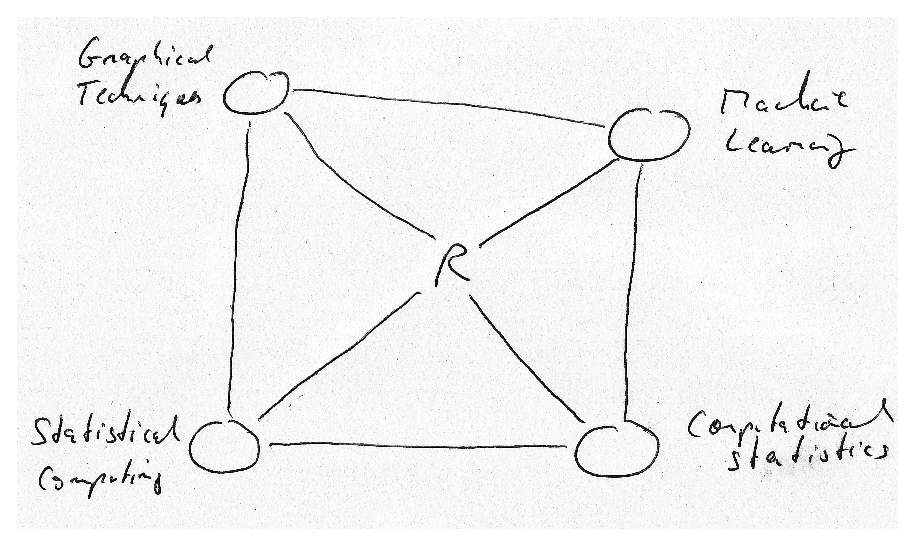
\includegraphics[height=40mm]{figures/techniques.eps}
\end{center}
\begin{description}
\item[Graphical Techniques:] scatter plots, histograms
\item[Statistical Computing:] hypothesis testing, linear regression, generalized linear models
\item[Computational Statistics:] bootstrap, monte carlo
\item[Machine Learning:] computational model building
\item[R:] statistical computing environment supporting all of the above activities
\end{description}
\es
\end{document}
%%%%%%%%%%%%%%%%%%%%%%%%%%% end of template1.tex %%%%%%%%%%%%%%%%%%%%%%%%%%%%%%%%

